\chapterimage{head2.png} % Chapter heading image
\chapter{EM Algorithm}

\section{The General EM Algorithm}
\begin{definition}[The joint probability]
    \begin{equation}
        p(\textbf{x}, \textbf{y})= p(x_0)\prod_{t=1}^{T} p(x_{t}|x_{t-1}) p(y_t|x_t)
    \end{equation}
    \begin{center}
        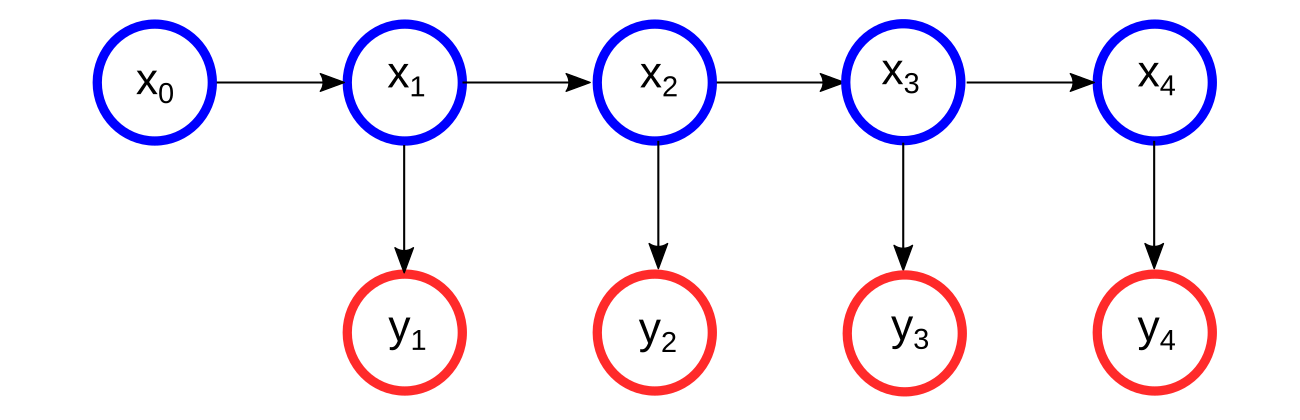
\includegraphics[scale=0.6]{ch2/four_states_ex.png}   
    \end{center}
In this example
    \begin{equation}
    \begin{split}
        p(\textbf{x}, \textbf{y})= &[p(x_0) p(x_1|x_0) p(y_1|x_1)] [p(x_2|x_1) p(y_2|x_2)]  [p(x_3|x_2) p(y_3|x_3)] \\
        &[p(x_4|x_3) p(y_4|x_4)]
    \end{split}
    \end{equation}
\end{definition}

\begin{definition}[The likelihood functional]
\begin{equation}
    L[\theta] = p(\textbf{y};\theta) = \int d\textbf{x}p(\textbf{x}, \textbf{y})
\end{equation}
\end{definition}

\begin{definition}[The log-likelihood functional]
\begin{equation}
    l[\theta] = \ln{(\int d\textbf{x}p(\textbf{x}, \textbf{y}))}
\end{equation}
\end{definition}

\begin{definition}[Solve Euler-Lagrange equation]
Maximization for the optimal parameter set requires taking derivatives of the log-likelihood functional and solves the resulting Euler-Lagrange equation:
\begin{equation}
        \frac{\partial l[\theta]}{\partial \theta} = \frac{\partial}{\partial \theta} \ln{(\int d\textbf{x}p(\textbf{x}, \textbf{y}))} = 0
\end{equation}
We can further get
\begin{equation}
    \frac{\partial l[\theta]}{\partial \theta} =  \frac{\partial \ln{L[\theta]}}{\partial \theta} = \frac{1}{L[\theta]}\frac{\partial L[\theta]}{\partial \theta}
\end{equation}
Because we need to do maximization according to previous step($k$), we want to solve the
following equation
\begin{equation}
    0 = \frac{\partial l^k[\theta]}{\partial \theta} = \frac{1}{L^k[\theta]}\frac{\partial L^k[\theta]}{\partial \theta}
\end{equation}
And we can express the likelihood functional as
\begin{equation}
    L^k[\theta] = p(\textbf{y}) = \sum_{\tau=0}^{T-1} \left<\alpha^k_{t_{\tau}}\right|  e^{-\textbf{H} \Delta t} \left|\beta^k_{t_{\tau+1}}\right>
\end{equation}
Therefore, the maximization problem becomes to solve
\begin{equation}
    0 =  \frac{\partial l^k[\theta]}{\partial \theta} = \frac{1}{L^k[\theta]} \sum_{\tau=0}^{T-1} \frac{\partial}{\partial \theta} \left<\alpha^k_{t_{\tau}}\right|  e^{-\textbf{H} \Delta t} \left|\beta^k_{t_{\tau+1}}\right>
\end{equation}
\end{definition}

\section{The expected log of the complete likelihood}
\begin{definition}[$\left<\alpha^k_{t_{0}}\right|  e^{-\textbf{H} \Delta t} \left|\beta^k_{t_{1}}\right>$]
\begin{equation}
    \left< \alpha_{t_0} | e^{-\textbf{H}\Delta t} | \beta_{t_1} \right> = \int p(x_0) p(x_1|x_0) p(y_2,y_3,y_4|x_1) dx_1= p(x_0,y_2,y_3,y_4)
\end{equation}
    \begin{center}
        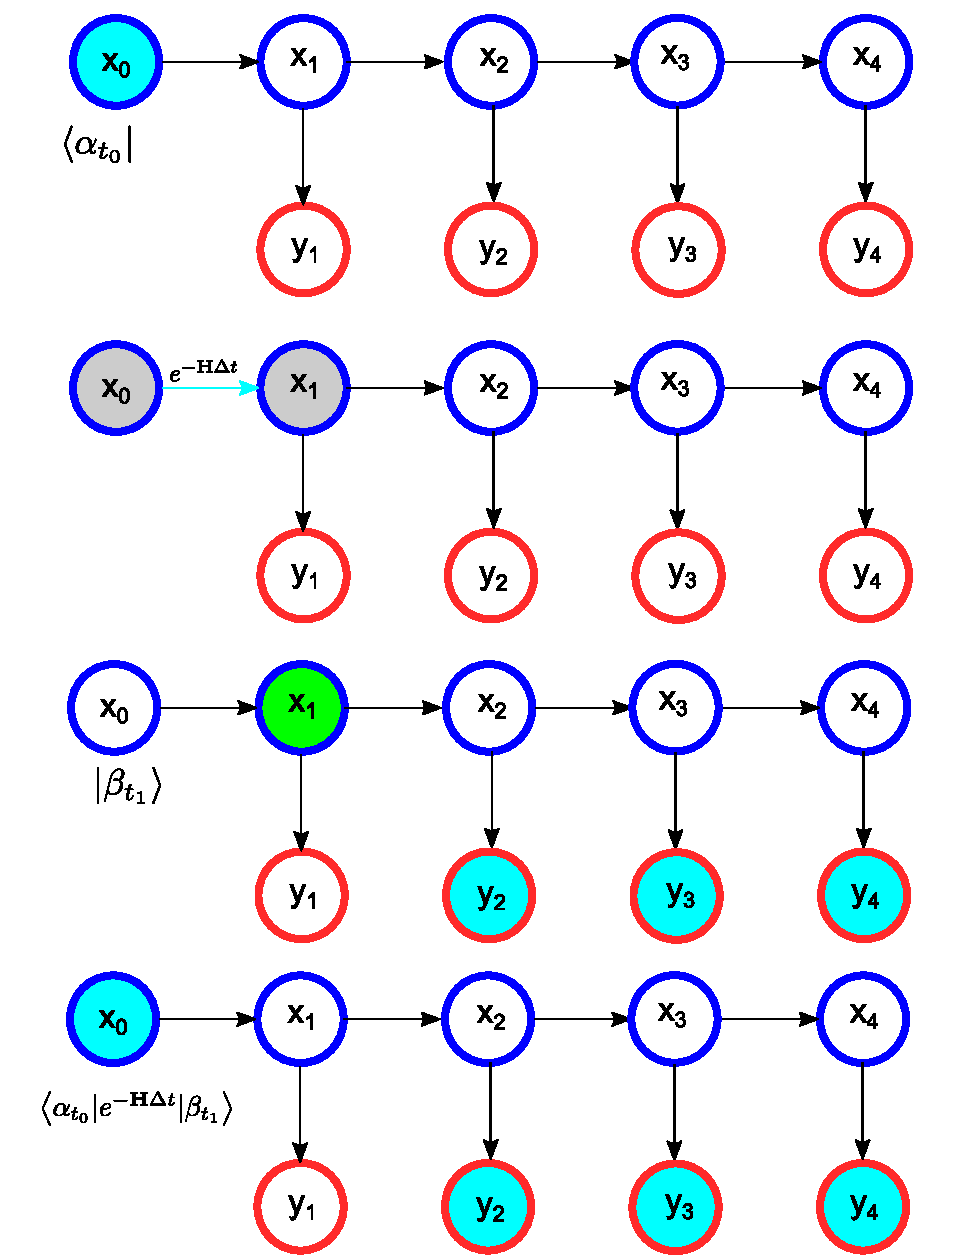
\includegraphics[scale=0.25]{ch4/alpha_t0_e_beta_t1.pdf}   
    \end{center}
\end{definition}

\begin{definition}[$\left<\alpha^k_{t_{1}}\right|  e^{-\textbf{H} \Delta t} \left|\beta^k_{t_{2}}\right>$]
\begin{equation}
    \left< \alpha_{t_1} | e^{-\textbf{H}\Delta t} | \beta_{t_2} \right> = \int p(x_1,y_1) p(x_2|x_1) p(y_3,y_4|x_2) dx_2= p(x_1,y_1,y_3,y_4)
\end{equation}
\begin{center}
    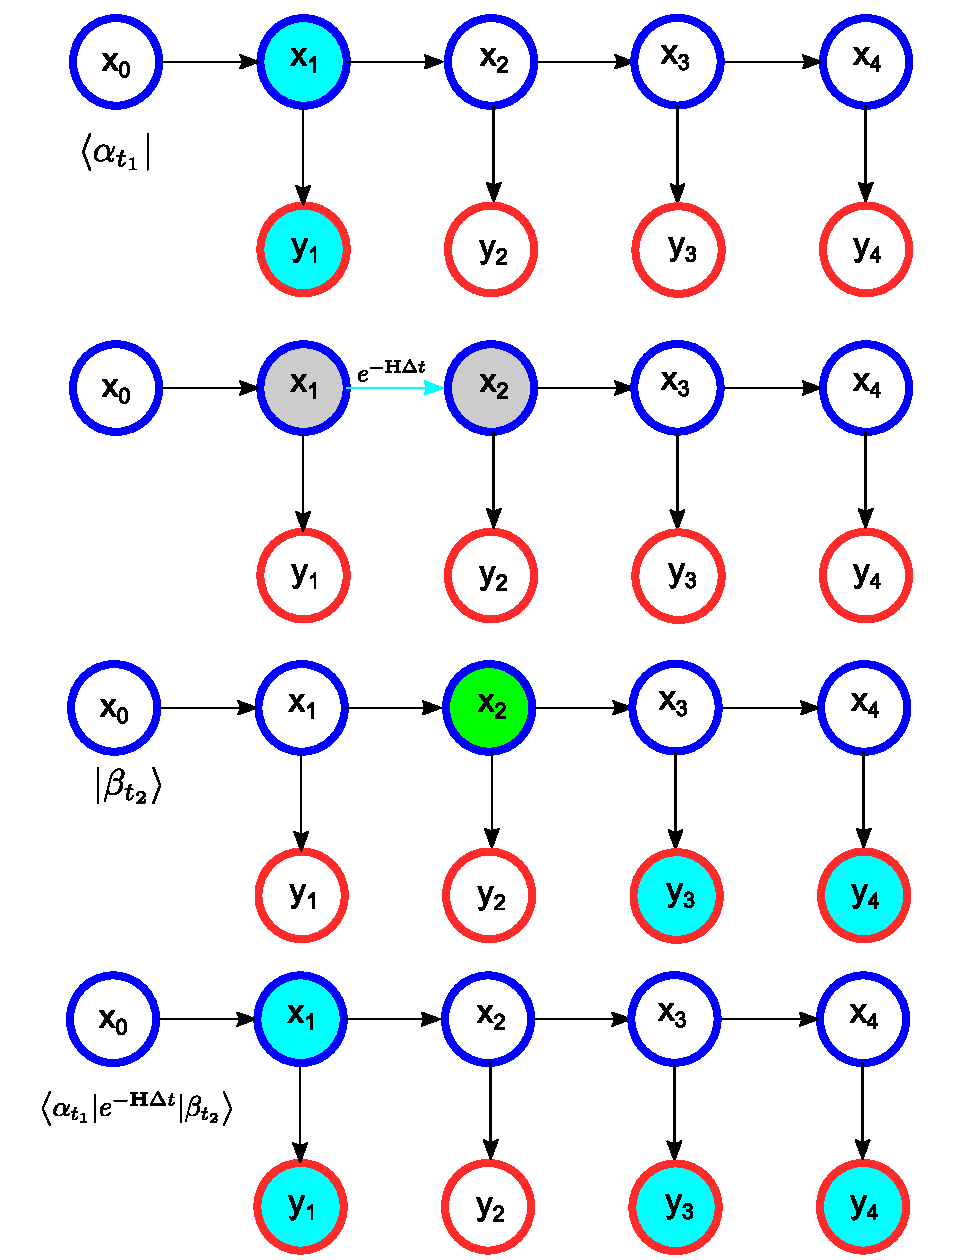
\includegraphics[scale=0.35]{ch4/alpha_t1_e_beta_t2.pdf}   
\end{center}
\end{definition}

\begin{definition}[$\left<\alpha^k_{t_{2}}\right|  e^{-\textbf{H} \Delta t} \left|\beta^k_{t_{3}}\right>$]
\begin{equation}
    \left< \alpha_{t_2} | e^{-\textbf{H}\Delta t} | \beta_{t_3} \right> = \int p(x_2,y_1,y_2) p(x_3|x_2) p(y_4|x_3) dx_3= p(x_2,y_1,y_2,y_4)
\end{equation}
\begin{center}
    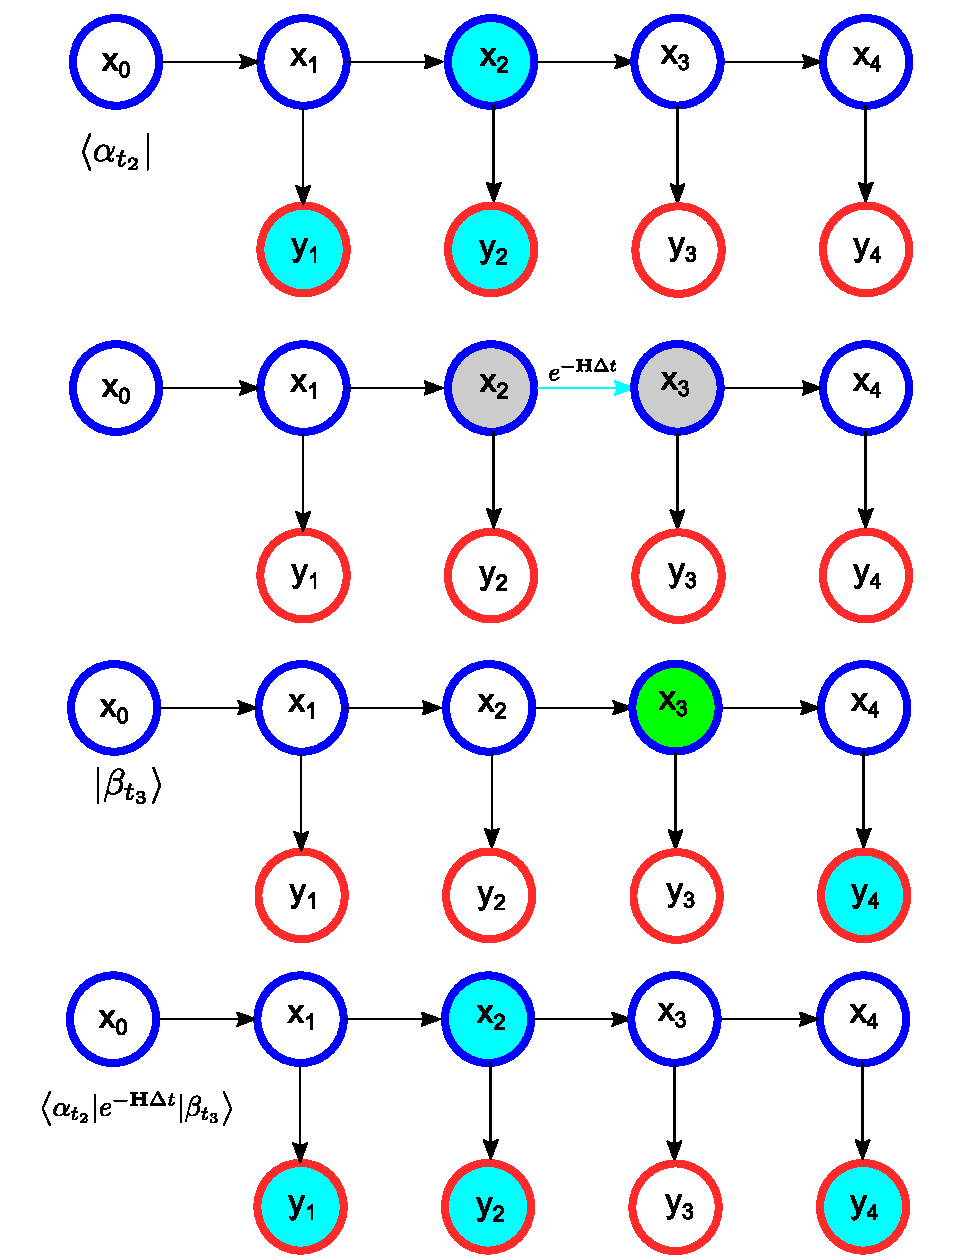
\includegraphics[scale=0.35]{ch4/alpha_t2_e_beta_t3.pdf}   
\end{center}
\end{definition}

\begin{definition}[$\left<\alpha^k_{t_{3}}\right|  e^{-\textbf{H} \Delta t} \left|\beta^k_{t_{4}}\right>$]
\begin{equation}
    \left< \alpha_{t_3} | e^{-\textbf{H}\Delta t} | \beta_{t_4} \right> = \int p(x_3,y_1,y_2,y_3) p(x_4|x_3) dx_4= p(x_3,y_1,y_2,y_3)
\end{equation}
\begin{center}
    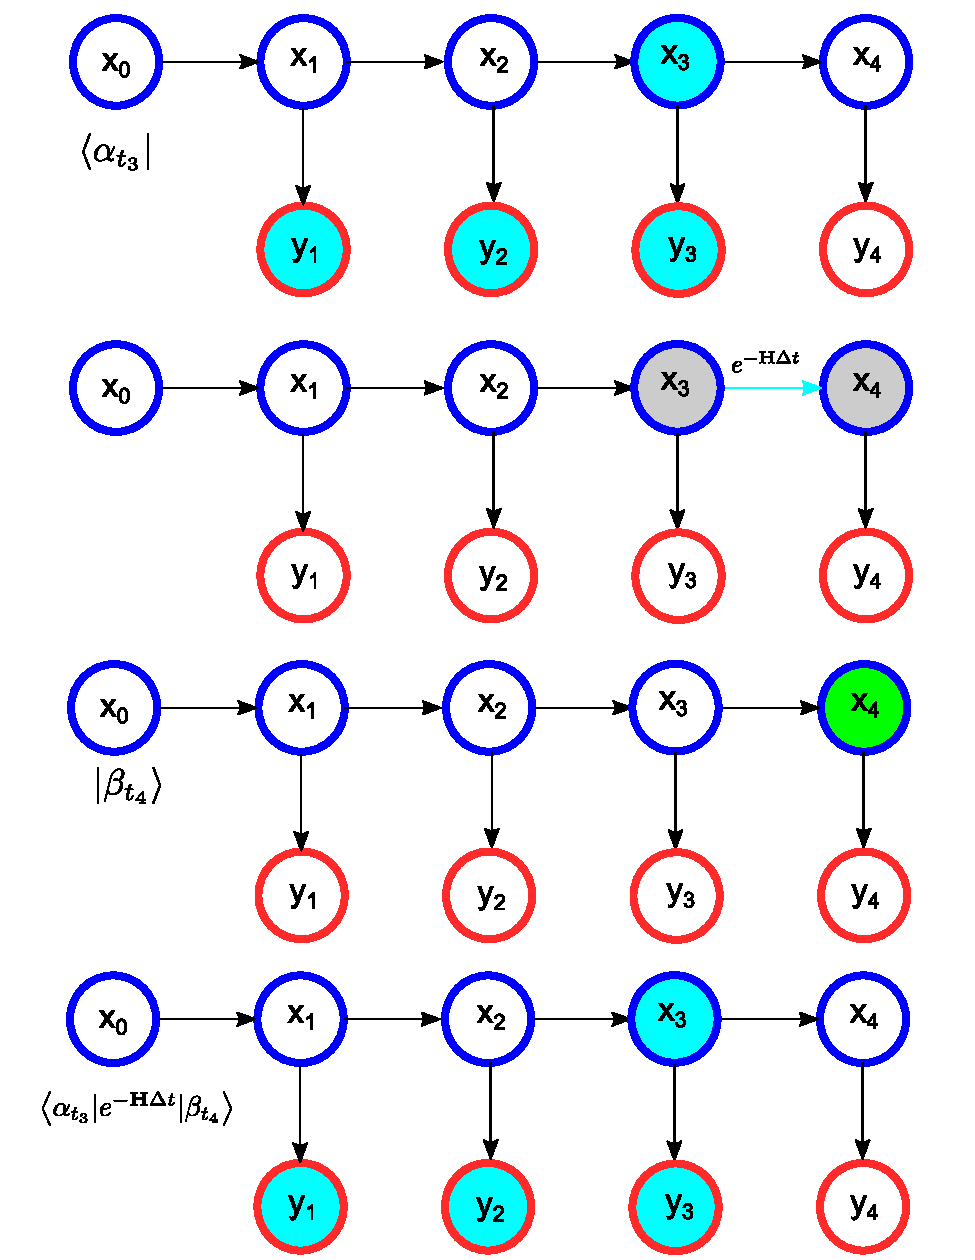
\includegraphics[scale=0.25]{ch4/alpha_t3_e_beta_t4.pdf}   
\end{center}
\end{definition}

\section{Update the equilibrium probability density}
\begin{definition}
    The basis functions in Def.(\ref{basisfunctions}) were used to update
\begin{align}
    p_{\rm eq}^{k+1}(x) &=\mathbb{E}^k_{X|Y} \left[ \delta(x-X) \right] \\
    &= p^k_{\rm{eq}}(x) \sum_{i,j} \mathbb{E}^k_{X|Y}[a_ib_j] \phi_i(x)\phi_j(x) \\
    &= \sum_{i,j} \psi_i(x) \mathbb{E}^k_{X|Y}[a_ib_j] \psi_j(x).
\end{align}
\end{definition}

\begin{definition}[Update from matrix multiplication]
\begin{align}
    p_{\rm eq}^{k+1}(x) = \mathrm{diag}(\Psi \mathbb{E}^k_{X|Y}[a_ib_j] \Psi^{\dagger})
\end{align}
\end{definition}

\begin{example}[$N_v=3$] In the matrix multiplication, I abbreviate $\mathbb{E}^k_{X|Y}[a_ib_j]$ as $a_ib_j$, and the grids are set like the bottom figure. We will show
\begin{align*}
    p_{\rm eq}^{k+1}(x) &=\sum_{i,j} \psi_i(x) \mathbb{E}^k_{X|Y}[a_ib_j] \psi_j(x) \\
    &= \mathrm{diag}(\Psi \mathbb{E}^k_{X|Y}[a_ib_j] \Psi^{\dagger})
\end{align*}
\begin{center}
    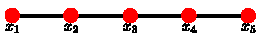
\includegraphics[scale=1.5]{ch4/ex1_grids.pdf}   
\end{center}
\begin{align*} 
&\Psi \mathbb{E}^k_{X|Y}[a_ib_j] \Psi^{\dagger} = \\
&\begin{bmatrix}
    \psi_1(x_1) & \psi_2(x_1) & \psi_3(x_1)  \\
    \psi_1(x_2) & \psi_2(x_2) & \psi_3(x_2) \\
    \psi_1(x_3) & \psi_2(x_3) & \psi_3(x_3)  \\
    \psi_1(x_4) & \psi_2(x_4) & \psi_3(x_4)  \\
    \psi_1(x_5) & \psi_2(x_5) & \psi_3(x_5)  
\end{bmatrix}
\begin{bmatrix}
    a_1 b_1 & a_1 b_2 & a_1 b_3  \\
    a_2 b_1 & a_2 b_2 & a_2 b_3 \\
    a_3 b_1 & a_3 b_2 & a_3 b_3
\end{bmatrix}
\begin{bmatrix}
    \psi_1(x_1) & \psi_1(x_2) & \psi_1(x_3) & \psi_1(x_4) & \psi_1(x_5) \\
    \psi_2(x_1) & \psi_2(x_2) & \psi_2(x_3) & \psi_2(x_4) & \psi_2(x_5) \\
    \psi_3(x_1) & \psi_3(x_2) & \psi_3(x_3) & \psi_3(x_4) & \psi_3(x_5) 
\end{bmatrix} \\
&=\begin{bmatrix}
    \sum_{i=1}^{3}a_i b_1 \psi_i(x_1) & \sum_{i=1}^{3}a_i b_2 \psi_i(x_1) & \sum_{i=1}^{3}a_i b_3 \psi_i(x_1) \\
    \sum_{i=1}^{3}a_i b_1 \psi_i(x_2) & \sum_{i=1}^{3}a_i b_2 \psi_i(x_2) & \sum_{i=1}^{3}a_i b_3 \psi_i(x_2) \\
    \sum_{i=1}^{3}a_i b_1 \psi_i(x_3) & \sum_{i=1}^{3}a_i b_2 \psi_i(x_3) & \sum_{i=1}^{3}a_i b_3 \psi_i(x_3) \\
    \sum_{i=1}^{3}a_i b_1 \psi_i(x_4) & \sum_{i=1}^{3}a_i b_2 \psi_i(x_4) & \sum_{i=1}^{3}a_i b_3 \psi_i(x_4) \\
    \sum_{i=1}^{3}a_i b_1 \psi_i(x_5) & \sum_{i=1}^{3}a_i b_2 \psi_i(x_5) & \sum_{i=1}^{3}a_i b_3 \psi_i(x_5) 
\end{bmatrix}\\
&\begin{bmatrix}
    \psi_1(x_1) & \psi_1(x_2) & \psi_1(x_3) & \psi_1(x_4) & \psi_1(x_5) \\
    \psi_2(x_1) & \psi_2(x_2) & \psi_2(x_3) & \psi_2(x_4) & \psi_2(x_5) \\
    \psi_3(x_1) & \psi_3(x_2) & \psi_3(x_3) & \psi_3(x_4) & \psi_3(x_5) 
\end{bmatrix}\\
&=
\begin{bmatrix}
\sum_{j=1}^{3} b_j \psi_j(x_1) \sum_{i=1}^{3}a_i \psi_i(x_1) &  \sum_{j=1}^{3} b_j \psi_j(x_2) \sum_{i=1}^{3}a_i \psi_i(x_1) &
\cdots & \sum_{j=1}^{3} b_j \psi_j(x_5) \sum_{i=1}^{3}a_i \psi_i(x_1) \\
\sum_{j=1}^{3} b_j \psi_j(x_1) \sum_{i=1}^{3}a_i \psi_i(x_2) &  \sum_{j=1}^{3} b_j \psi_j(x_2) \sum_{i=1}^{3}a_i \psi_i(x_2) &
\cdots & \sum_{j=1}^{3} b_j \psi_j(x_5) \sum_{i=1}^{3}a_i \psi_i(x_2) \\
\sum_{j=1}^{3} b_j \psi_j(x_1) \sum_{i=1}^{3}a_i \psi_i(x_3) &  \sum_{j=1}^{3} b_j \psi_j(x_2) \sum_{i=1}^{3}a_i \psi_i(x_3) &
\cdots & \sum_{j=1}^{3} b_j \psi_j(x_5) \sum_{i=1}^{3}a_i \psi_i(x_3) \\
\sum_{j=1}^{3} b_j \psi_j(x_1) \sum_{i=1}^{3}a_i \psi_i(x_4) &  \sum_{j=1}^{3} b_j \psi_j(x_2) \sum_{i=1}^{3}a_i \psi_i(x_4) &
\cdots & \sum_{j=1}^{3} b_j \psi_j(x_5) \sum_{i=1}^{3}a_i \psi_i(x_4) \\
\sum_{j=1}^{3} b_j \psi_j(x_1) \sum_{i=1}^{3}a_i \psi_i(x_5) &  \sum_{j=1}^{3} b_j \psi_j(x_2) \sum_{i=1}^{3}a_i \psi_i(x_5) &
\cdots & \sum_{j=1}^{3} b_j \psi_j(x_5) \sum_{i=1}^{3}a_i \psi_i(x_5)
\end{bmatrix}
\end{align*}
\end{example}

\section{EM Test}
\begin{center}
    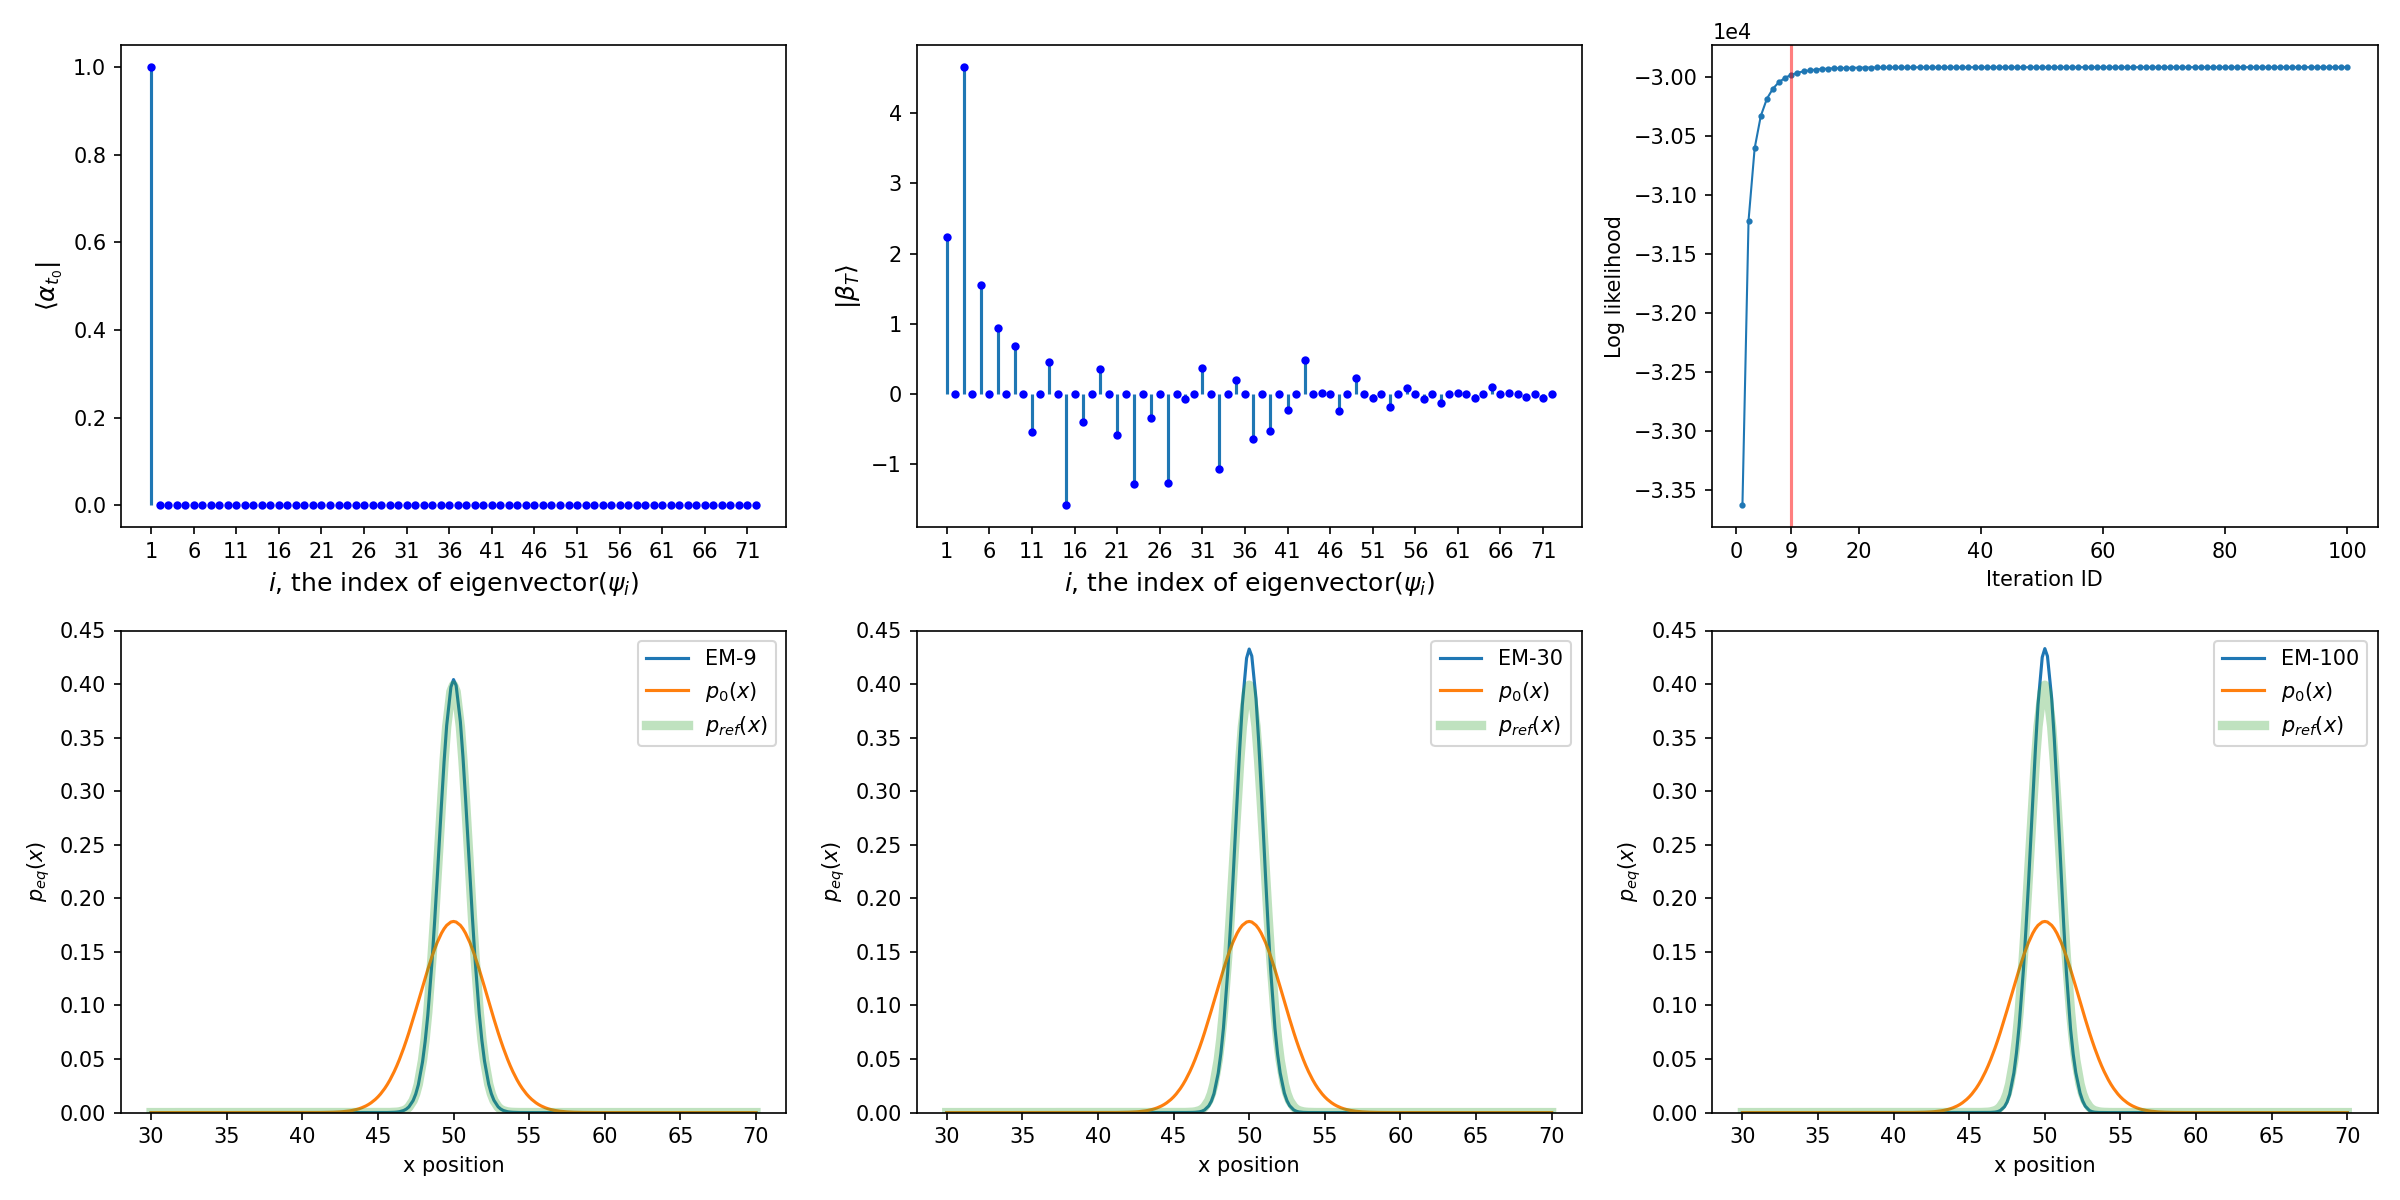
\includegraphics[scale=0.36]{ch4/forward_backward_v2.png}   
\end{center}